%------------------------------------------------------------------------
\begin{frame}
	\frametitle{Content}
	\framesubtitle{ABS-Normal Form}
	\begin{columns}[T] % align columns
		\begin{column}{.48\textwidth}
			
			\begin{center}
				{\Huge Blocksize und \\ Gridsize?}
			\end{center}
			
		\end{column}%
		\hfill%
		\begin{column}{.48\textwidth}
			\color{blue}\rule{\linewidth}{4pt}
			
			\setbeamertemplate{enumerate items}[default]
			\begin{enumerate}
				\item Einführung
				\item Aufgaben
				\item Evaluate
				\item Gradient
				\item Blocksize und Gridsize
				\item Solve
				\item Final Thoughts
			\end{enumerate}
		\end{column}%
	\end{columns}
\end{frame}
%------------------------------------------------------------------------
\begin{frame}
	\frametitle{Choosing Gridsize and Blocksize}
	\framesubtitle{Ansatz}
	Wie sollen gridsize and blocksize gewählt werden?
	\begin{itemize}
		\item <2-> Generischen Ansatz
		\item <3-> Starte mit gewisser blocksize and gridsize in abh. von device spec.
		\item <4-> threads berechnen, welche aufgaben sie abarbeiten sollen
		\item <5-> über die optimalen parameter kann optimiert werden.
	\end{itemize}
\end{frame}
%------------------------------------------------------------------------
\begin{frame}[fragile]
	\frametitle{Choosing Gridsize and Blocksize}
	\framesubtitle{Beispiel}
	Zu Implementierende Operation:
	\begin{flalign*}
	A = A \times Diag(Sign(dz))
	\end{flalign*}
	\pause
	Beispiel:
	\begin{flalign*}
	A \in \mathbb{R}^{3 \times 3}, dz \in \mathbb{R}^2 \\
	\end{flalign*}
	\begin{flalign*}
			dz = (-j, 0, k)
	\end{flalign*}
	\begin{flalign*}
	\left(\begin{array}{ccc}
	a & d & g \\
	b & e & h \\
	c & f & i \\
	\end{array}\right) \times
	\left(\begin{array}{ccc}
	-1 & 0 & 0 \\
	0 & 0 & 0 \\
	0 & 0 & 1 \\
	\end{array}\right)
	=
	\left(\begin{array}{ccc}
	-a & 0 & g \\
	-b & 0 & h \\
	-c & 0 & i \\
	\end{array}\right)
	\end{flalign*}
\end{frame}
%------------------------------------------------------------------------
\begin{frame}[fragile]
	\frametitle{Choosing Gridsize and Blocksize}
	\framesubtitle{Beispiel}
	\begin{center}
		ANIMATION
	\end{center}
\end{frame}
%------------------------------------------------------------------------
\begin{frame}[fragile]
	\frametitle{Choosing Gridsize and Blocksize}
	\framesubtitle{Beispiel - Implementierung}
	\begin{lstlisting}[language=cpp]
	template <typename T>
	void __global__ multWithDz(T *A, T *dz, int s){
		int i = threadIdx.x;
		int j = blockIdx.x;
		int id = i*s + j;
		while(id < s*s && j < s){
			if(i<s){
				if(A[id] != T(0)) 
					A[id] = A[id] * cuutils::sign(&dz[j]);
				i+=blockDim.x;
			}
			else{
				i = i%s;
				j = j + gridDim.x;
			}
			id = i*s + j;
		}			
	}
	\end{lstlisting}
\end{frame}
%------------------------------------------------------------------------

\setbeamertemplate{navigation symbols}{}
\begin{frame}[plain]
	\makebox[\linewidth]{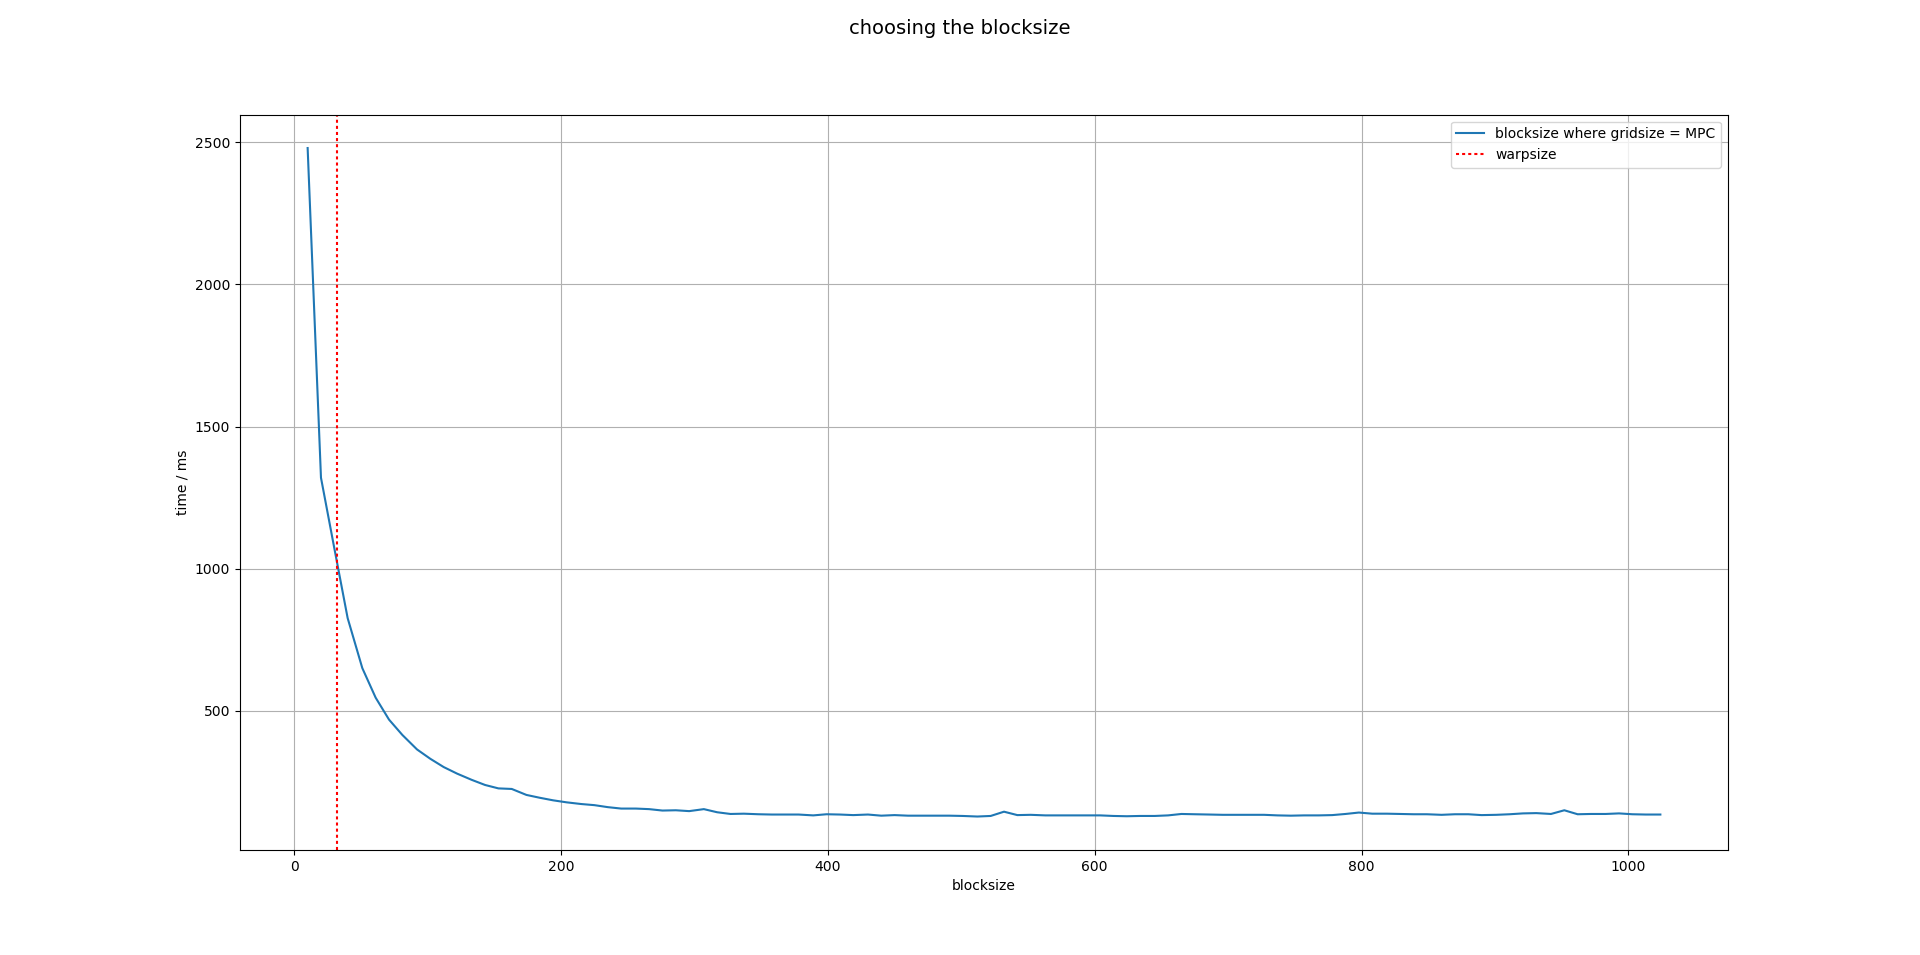
\includegraphics[width=\paperwidth]{img/blocksize.png}}
\end{frame}
\setbeamertemplate{navigation symbols}{}
\begin{frame}[plain]
	\makebox[\linewidth]{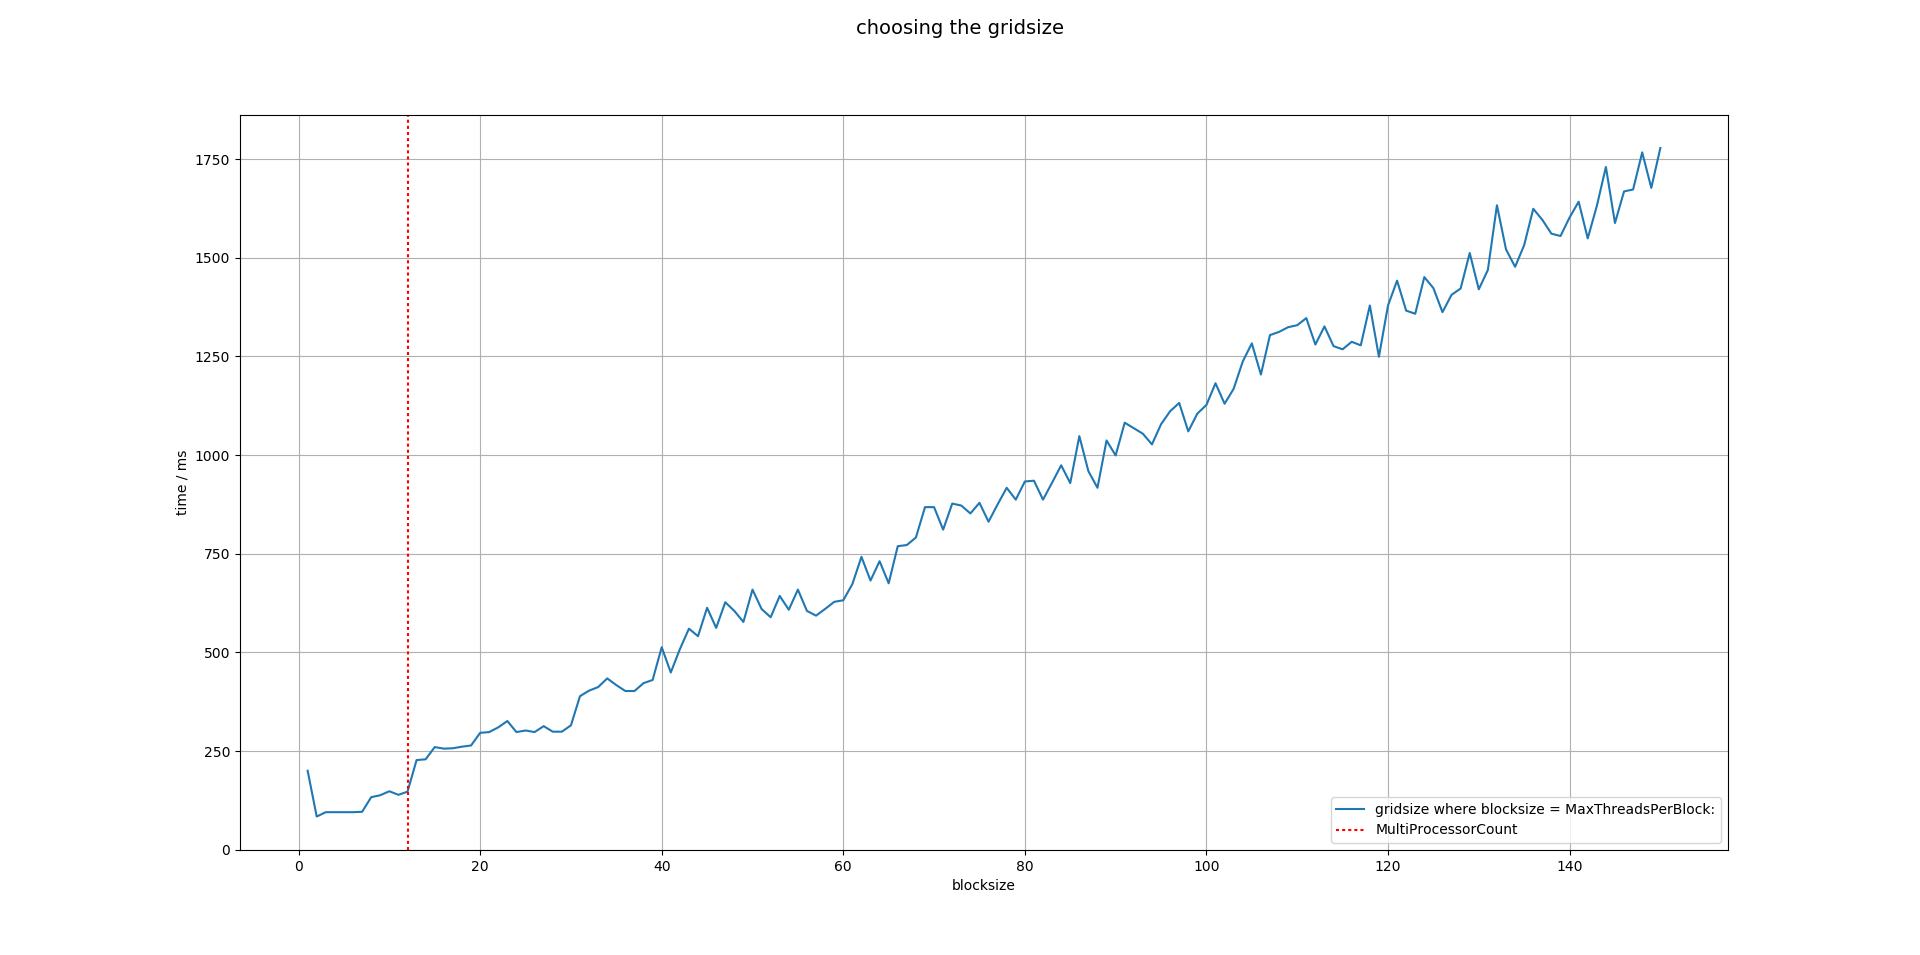
\includegraphics[width=\paperwidth]{img/gridsize.png}}
\end{frame}
\begin{frame}[plain]
	\makebox[\linewidth]{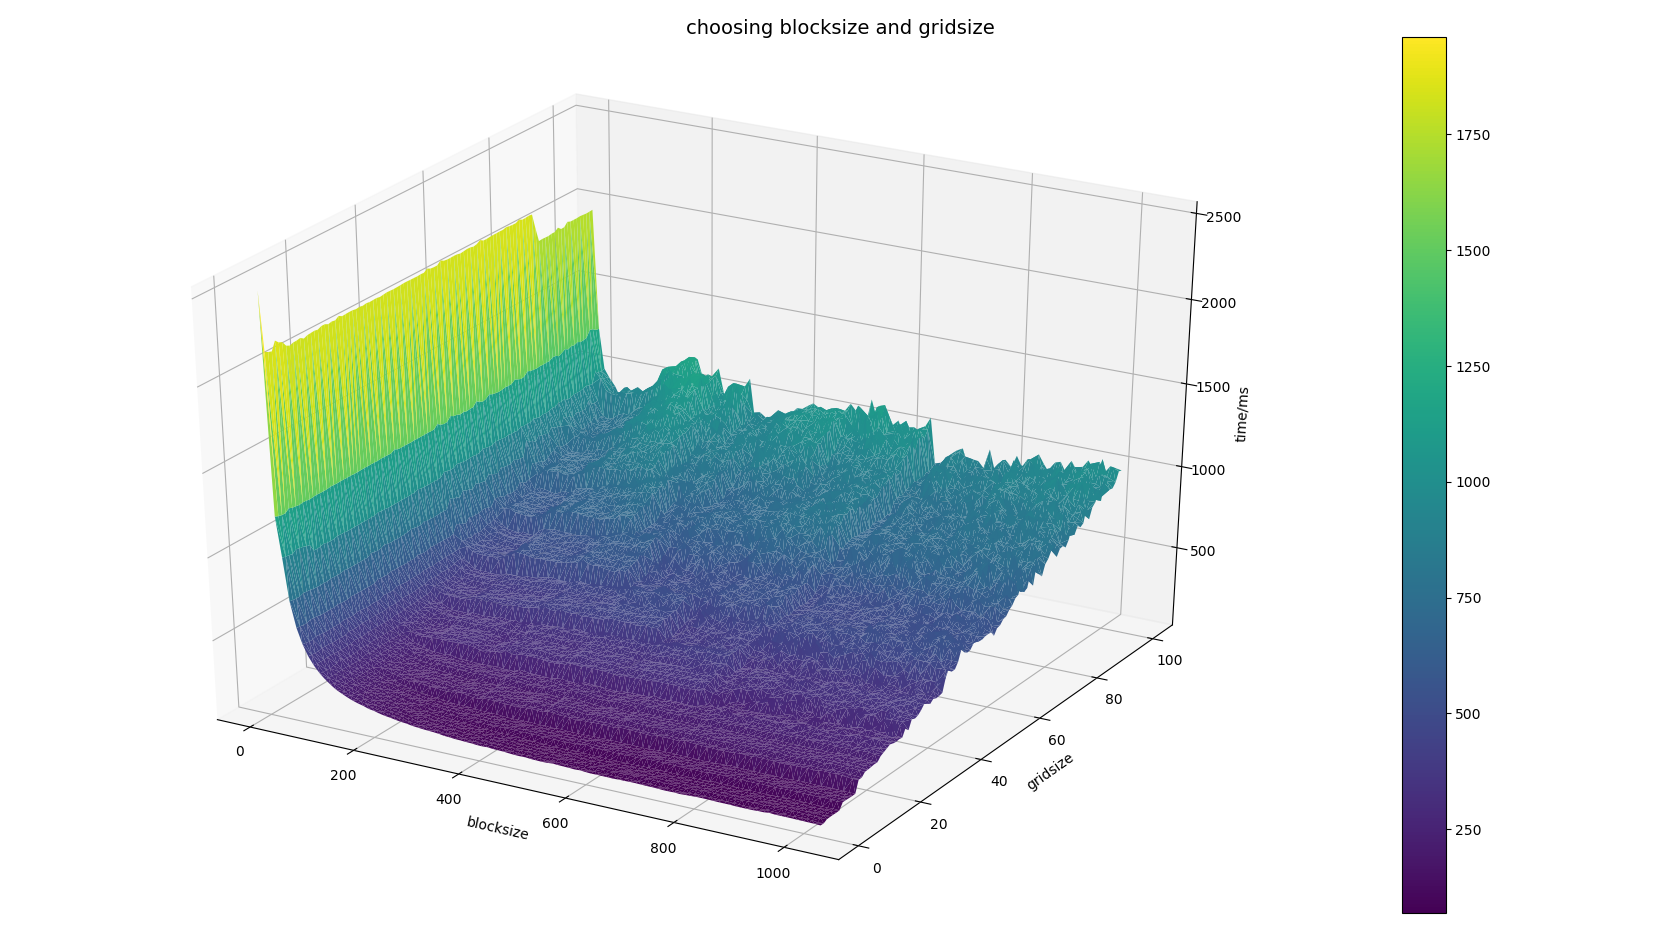
\includegraphics[width=\paperwidth]{img/block_grid_3d.png}}
\end{frame}